% Options for packages loaded elsewhere
\PassOptionsToPackage{unicode}{hyperref}
\PassOptionsToPackage{hyphens}{url}
%
\documentclass[
]{book}
\usepackage{lmodern}
\usepackage{amsmath}
\usepackage{ifxetex,ifluatex}
\ifnum 0\ifxetex 1\fi\ifluatex 1\fi=0 % if pdftex
  \usepackage[T1]{fontenc}
  \usepackage[utf8]{inputenc}
  \usepackage{textcomp} % provide euro and other symbols
  \usepackage{amssymb}
\else % if luatex or xetex
  \usepackage{unicode-math}
  \defaultfontfeatures{Scale=MatchLowercase}
  \defaultfontfeatures[\rmfamily]{Ligatures=TeX,Scale=1}
\fi
% Use upquote if available, for straight quotes in verbatim environments
\IfFileExists{upquote.sty}{\usepackage{upquote}}{}
\IfFileExists{microtype.sty}{% use microtype if available
  \usepackage[]{microtype}
  \UseMicrotypeSet[protrusion]{basicmath} % disable protrusion for tt fonts
}{}
\makeatletter
\@ifundefined{KOMAClassName}{% if non-KOMA class
  \IfFileExists{parskip.sty}{%
    \usepackage{parskip}
  }{% else
    \setlength{\parindent}{0pt}
    \setlength{\parskip}{6pt plus 2pt minus 1pt}}
}{% if KOMA class
  \KOMAoptions{parskip=half}}
\makeatother
\usepackage{xcolor}
\IfFileExists{xurl.sty}{\usepackage{xurl}}{} % add URL line breaks if available
\IfFileExists{bookmark.sty}{\usepackage{bookmark}}{\usepackage{hyperref}}
\hypersetup{
  pdftitle={Applied regression analysis},
  pdfauthor={Andrew Li},
  hidelinks,
  pdfcreator={LaTeX via pandoc}}
\urlstyle{same} % disable monospaced font for URLs
\usepackage{color}
\usepackage{fancyvrb}
\newcommand{\VerbBar}{|}
\newcommand{\VERB}{\Verb[commandchars=\\\{\}]}
\DefineVerbatimEnvironment{Highlighting}{Verbatim}{commandchars=\\\{\}}
% Add ',fontsize=\small' for more characters per line
\usepackage{framed}
\definecolor{shadecolor}{RGB}{248,248,248}
\newenvironment{Shaded}{\begin{snugshade}}{\end{snugshade}}
\newcommand{\AlertTok}[1]{\textcolor[rgb]{0.94,0.16,0.16}{#1}}
\newcommand{\AnnotationTok}[1]{\textcolor[rgb]{0.56,0.35,0.01}{\textbf{\textit{#1}}}}
\newcommand{\AttributeTok}[1]{\textcolor[rgb]{0.77,0.63,0.00}{#1}}
\newcommand{\BaseNTok}[1]{\textcolor[rgb]{0.00,0.00,0.81}{#1}}
\newcommand{\BuiltInTok}[1]{#1}
\newcommand{\CharTok}[1]{\textcolor[rgb]{0.31,0.60,0.02}{#1}}
\newcommand{\CommentTok}[1]{\textcolor[rgb]{0.56,0.35,0.01}{\textit{#1}}}
\newcommand{\CommentVarTok}[1]{\textcolor[rgb]{0.56,0.35,0.01}{\textbf{\textit{#1}}}}
\newcommand{\ConstantTok}[1]{\textcolor[rgb]{0.00,0.00,0.00}{#1}}
\newcommand{\ControlFlowTok}[1]{\textcolor[rgb]{0.13,0.29,0.53}{\textbf{#1}}}
\newcommand{\DataTypeTok}[1]{\textcolor[rgb]{0.13,0.29,0.53}{#1}}
\newcommand{\DecValTok}[1]{\textcolor[rgb]{0.00,0.00,0.81}{#1}}
\newcommand{\DocumentationTok}[1]{\textcolor[rgb]{0.56,0.35,0.01}{\textbf{\textit{#1}}}}
\newcommand{\ErrorTok}[1]{\textcolor[rgb]{0.64,0.00,0.00}{\textbf{#1}}}
\newcommand{\ExtensionTok}[1]{#1}
\newcommand{\FloatTok}[1]{\textcolor[rgb]{0.00,0.00,0.81}{#1}}
\newcommand{\FunctionTok}[1]{\textcolor[rgb]{0.00,0.00,0.00}{#1}}
\newcommand{\ImportTok}[1]{#1}
\newcommand{\InformationTok}[1]{\textcolor[rgb]{0.56,0.35,0.01}{\textbf{\textit{#1}}}}
\newcommand{\KeywordTok}[1]{\textcolor[rgb]{0.13,0.29,0.53}{\textbf{#1}}}
\newcommand{\NormalTok}[1]{#1}
\newcommand{\OperatorTok}[1]{\textcolor[rgb]{0.81,0.36,0.00}{\textbf{#1}}}
\newcommand{\OtherTok}[1]{\textcolor[rgb]{0.56,0.35,0.01}{#1}}
\newcommand{\PreprocessorTok}[1]{\textcolor[rgb]{0.56,0.35,0.01}{\textit{#1}}}
\newcommand{\RegionMarkerTok}[1]{#1}
\newcommand{\SpecialCharTok}[1]{\textcolor[rgb]{0.00,0.00,0.00}{#1}}
\newcommand{\SpecialStringTok}[1]{\textcolor[rgb]{0.31,0.60,0.02}{#1}}
\newcommand{\StringTok}[1]{\textcolor[rgb]{0.31,0.60,0.02}{#1}}
\newcommand{\VariableTok}[1]{\textcolor[rgb]{0.00,0.00,0.00}{#1}}
\newcommand{\VerbatimStringTok}[1]{\textcolor[rgb]{0.31,0.60,0.02}{#1}}
\newcommand{\WarningTok}[1]{\textcolor[rgb]{0.56,0.35,0.01}{\textbf{\textit{#1}}}}
\usepackage{longtable,booktabs}
\usepackage{calc} % for calculating minipage widths
% Correct order of tables after \paragraph or \subparagraph
\usepackage{etoolbox}
\makeatletter
\patchcmd\longtable{\par}{\if@noskipsec\mbox{}\fi\par}{}{}
\makeatother
% Allow footnotes in longtable head/foot
\IfFileExists{footnotehyper.sty}{\usepackage{footnotehyper}}{\usepackage{footnote}}
\makesavenoteenv{longtable}
\usepackage{graphicx}
\makeatletter
\def\maxwidth{\ifdim\Gin@nat@width>\linewidth\linewidth\else\Gin@nat@width\fi}
\def\maxheight{\ifdim\Gin@nat@height>\textheight\textheight\else\Gin@nat@height\fi}
\makeatother
% Scale images if necessary, so that they will not overflow the page
% margins by default, and it is still possible to overwrite the defaults
% using explicit options in \includegraphics[width, height, ...]{}
\setkeys{Gin}{width=\maxwidth,height=\maxheight,keepaspectratio}
% Set default figure placement to htbp
\makeatletter
\def\fps@figure{htbp}
\makeatother
\setlength{\emergencystretch}{3em} % prevent overfull lines
\providecommand{\tightlist}{%
  \setlength{\itemsep}{0pt}\setlength{\parskip}{0pt}}
\setcounter{secnumdepth}{5}
\usepackage{booktabs}
\usepackage{amsthm}
\makeatletter
\def\thm@space@setup{%
  \thm@preskip=8pt plus 2pt minus 4pt
  \thm@postskip=\thm@preskip
}
\makeatother
\ifluatex
  \usepackage{selnolig}  % disable illegal ligatures
\fi
\usepackage[]{natbib}
\bibliographystyle{apalike}

\title{Applied regression analysis}
\author{Andrew Li}
\date{Spring 2021}

\begin{document}
\maketitle

{
\setcounter{tocdepth}{1}
\tableofcontents
}
\hypertarget{preamble}{%
\chapter{Preamble}\label{preamble}}

\hypertarget{caution}{%
\section{Caution}\label{caution}}

\textbf{This book was made for studying purposes only.} I will be adding notes from other sources and I may leave out some topics from the course. Also, I will not be purchasing or reading the supplemental text. As such, this is not a faithful representation of the course.

\hypertarget{acknowledgments}{%
\section{Acknowledgments}\label{acknowledgments}}

This course was taught by \href{https://psych.ubc.ca/profile/jason-rights/}{Dr.~Jason Rights}!

\hypertarget{course-goals}{%
\section{Course goals}\label{course-goals}}

There are three primary goals of this course. The first goal is to provide students with sound foundational knowledge in the theory and concepts of linear regression analysis. The second goal is to develop an ability to properly apply regression methods to empirical data, including making informed decisions about analytic strategies and understanding how to report results. The third goal is to be able to critically evaluate the use of linear regression methods in research literature and the news. This course requires the successful completion of PSYC 218.

\hypertarget{readings}{%
\section{Readings}\label{readings}}

\begin{itemize}
\tightlist
\item
  Supplemental textbook (not required): Cohen, J., Cohen, P., West, S. G., \& Aiken, L. S. (2003). \emph{Applied multiple regression/correlation analysis for the behavioral sciences.} (3rd edition). Hillsdale, NJ: Erlbaum.
\end{itemize}

\hypertarget{course-content}{%
\section{Course content}\label{course-content}}

\textbf{Note:} Bolded weeks indicates that a problem set is due or there is a midterm.

\begin{longtable}[]{@{}lllll@{}}
\toprule
\begin{minipage}[b]{(\columnwidth - 4\tabcolsep) * \real{0.05}}\raggedright
Week\strut
\end{minipage} & \begin{minipage}[b]{(\columnwidth - 4\tabcolsep) * \real{0.08}}\raggedright
Date (2021)\strut
\end{minipage} & \begin{minipage}[b]{(\columnwidth - 4\tabcolsep) * \real{0.57}}\raggedright
Lecture topics\strut
\end{minipage} & \begin{minipage}[b]{(\columnwidth - 4\tabcolsep) * \real{0.27}}\raggedright
Readings\strut
\end{minipage} & \begin{minipage}[b]{(\columnwidth - 4\tabcolsep) * \real{0.04}}\raggedright
HW/MT\strut
\end{minipage}\tabularnewline
\midrule
\endhead
\begin{minipage}[t]{(\columnwidth - 4\tabcolsep) * \real{0.05}}\raggedright
1\strut
\end{minipage} & \begin{minipage}[t]{(\columnwidth - 4\tabcolsep) * \real{0.08}}\raggedright
1/11 - 1/15\strut
\end{minipage} & \begin{minipage}[t]{(\columnwidth - 4\tabcolsep) * \real{0.57}}\raggedright
1. Orientation; Review of the Pearson correlation2. Factor affecting the size of correlation\strut
\end{minipage} & \begin{minipage}[t]{(\columnwidth - 4\tabcolsep) * \real{0.27}}\raggedright
1. (Ch. 1, 2.1 - 2.2) 2. (Ch. 2.3: 2.10)\strut
\end{minipage} & \begin{minipage}[t]{(\columnwidth - 4\tabcolsep) * \real{0.04}}\raggedright
none\strut
\end{minipage}\tabularnewline
\begin{minipage}[t]{(\columnwidth - 4\tabcolsep) * \real{0.05}}\raggedright
2\strut
\end{minipage} & \begin{minipage}[t]{(\columnwidth - 4\tabcolsep) * \real{0.08}}\raggedright
1/18 - 1/22\strut
\end{minipage} & \begin{minipage}[t]{(\columnwidth - 4\tabcolsep) * \real{0.57}}\raggedright
1. Simple linear regression 2. Inferences for SLR\strut
\end{minipage} & \begin{minipage}[t]{(\columnwidth - 4\tabcolsep) * \real{0.27}}\raggedright
1. (Ch. 2.4 - 2.7) 2. (Ch. 2.8)\strut
\end{minipage} & \begin{minipage}[t]{(\columnwidth - 4\tabcolsep) * \real{0.04}}\raggedright
none\strut
\end{minipage}\tabularnewline
\begin{minipage}[t]{(\columnwidth - 4\tabcolsep) * \real{0.05}}\raggedright
\textbf{3}\strut
\end{minipage} & \begin{minipage}[t]{(\columnwidth - 4\tabcolsep) * \real{0.08}}\raggedright
1/25 - 1/29\strut
\end{minipage} & \begin{minipage}[t]{(\columnwidth - 4\tabcolsep) * \real{0.57}}\raggedright
1. Multiple linear regression (MLR) with 2 IVs\strut
\end{minipage} & \begin{minipage}[t]{(\columnwidth - 4\tabcolsep) * \real{0.27}}\raggedright
(Ch. 3.1 - 3.2)\strut
\end{minipage} & \begin{minipage}[t]{(\columnwidth - 4\tabcolsep) * \real{0.04}}\raggedright
HW 1\strut
\end{minipage}\tabularnewline
\begin{minipage}[t]{(\columnwidth - 4\tabcolsep) * \real{0.05}}\raggedright
4\strut
\end{minipage} & \begin{minipage}[t]{(\columnwidth - 4\tabcolsep) * \real{0.08}}\raggedright
2/1 - 2/5\strut
\end{minipage} & \begin{minipage}[t]{(\columnwidth - 4\tabcolsep) * \real{0.57}}\raggedright
1. MLR with k IVs\strut
\end{minipage} & \begin{minipage}[t]{(\columnwidth - 4\tabcolsep) * \real{0.27}}\raggedright
(Ch. 3.5)\strut
\end{minipage} & \begin{minipage}[t]{(\columnwidth - 4\tabcolsep) * \real{0.04}}\raggedright
none\strut
\end{minipage}\tabularnewline
\begin{minipage}[t]{(\columnwidth - 4\tabcolsep) * \real{0.05}}\raggedright
\textbf{5}\strut
\end{minipage} & \begin{minipage}[t]{(\columnwidth - 4\tabcolsep) * \real{0.08}}\raggedright
2/8 - 2/12\strut
\end{minipage} & \begin{minipage}[t]{(\columnwidth - 4\tabcolsep) * \real{0.57}}\raggedright
\emph{Lecture catch-up}\strut
\end{minipage} & \begin{minipage}[t]{(\columnwidth - 4\tabcolsep) * \real{0.27}}\raggedright
none\strut
\end{minipage} & \begin{minipage}[t]{(\columnwidth - 4\tabcolsep) * \real{0.04}}\raggedright
MT1\strut
\end{minipage}\tabularnewline
\begin{minipage}[t]{(\columnwidth - 4\tabcolsep) * \real{0.05}}\raggedright
6\strut
\end{minipage} & \begin{minipage}[t]{(\columnwidth - 4\tabcolsep) * \real{0.08}}\raggedright
2/15 - 2/19\strut
\end{minipage} & \begin{minipage}[t]{(\columnwidth - 4\tabcolsep) * \real{0.57}}\raggedright
\emph{Spring Break}\strut
\end{minipage} & \begin{minipage}[t]{(\columnwidth - 4\tabcolsep) * \real{0.27}}\raggedright
none\strut
\end{minipage} & \begin{minipage}[t]{(\columnwidth - 4\tabcolsep) * \real{0.04}}\raggedright
none\strut
\end{minipage}\tabularnewline
\begin{minipage}[t]{(\columnwidth - 4\tabcolsep) * \real{0.05}}\raggedright
\textbf{7}\strut
\end{minipage} & \begin{minipage}[t]{(\columnwidth - 4\tabcolsep) * \real{0.08}}\raggedright
2/22 - 2/26\strut
\end{minipage} & \begin{minipage}[t]{(\columnwidth - 4\tabcolsep) * \real{0.57}}\raggedright
1. Power analysis for MLR 2. Hierarchical regression\strut
\end{minipage} & \begin{minipage}[t]{(\columnwidth - 4\tabcolsep) * \real{0.27}}\raggedright
1. (Ch. 3.7) 2. (Ch. 5.3)\strut
\end{minipage} & \begin{minipage}[t]{(\columnwidth - 4\tabcolsep) * \real{0.04}}\raggedright
HW2\strut
\end{minipage}\tabularnewline
\begin{minipage}[t]{(\columnwidth - 4\tabcolsep) * \real{0.05}}\raggedright
8\strut
\end{minipage} & \begin{minipage}[t]{(\columnwidth - 4\tabcolsep) * \real{0.08}}\raggedright
3/1 - 3/5\strut
\end{minipage} & \begin{minipage}[t]{(\columnwidth - 4\tabcolsep) * \real{0.57}}\raggedright
1. Interactions in MLR\strut
\end{minipage} & \begin{minipage}[t]{(\columnwidth - 4\tabcolsep) * \real{0.27}}\raggedright
(Ch. 7.1 -7.4)\strut
\end{minipage} & \begin{minipage}[t]{(\columnwidth - 4\tabcolsep) * \real{0.04}}\raggedright
none\strut
\end{minipage}\tabularnewline
\begin{minipage}[t]{(\columnwidth - 4\tabcolsep) * \real{0.05}}\raggedright
\textbf{9}\strut
\end{minipage} & \begin{minipage}[t]{(\columnwidth - 4\tabcolsep) * \real{0.08}}\raggedright
3/8 - 3/12\strut
\end{minipage} & \begin{minipage}[t]{(\columnwidth - 4\tabcolsep) * \real{0.57}}\raggedright
1. Assumptions in MLR: Definitions and testing\strut
\end{minipage} & \begin{minipage}[t]{(\columnwidth - 4\tabcolsep) * \real{0.27}}\raggedright
(Ch. 4.1 - 4.5)\strut
\end{minipage} & \begin{minipage}[t]{(\columnwidth - 4\tabcolsep) * \real{0.04}}\raggedright
HW3\strut
\end{minipage}\tabularnewline
\begin{minipage}[t]{(\columnwidth - 4\tabcolsep) * \real{0.05}}\raggedright
\textbf{10}\strut
\end{minipage} & \begin{minipage}[t]{(\columnwidth - 4\tabcolsep) * \real{0.08}}\raggedright
3/15 - 3/19\strut
\end{minipage} & \begin{minipage}[t]{(\columnwidth - 4\tabcolsep) * \real{0.57}}\raggedright
1. Categorical IVs: Dummy coding 2. Categorial IVs: Effect coding\strut
\end{minipage} & \begin{minipage}[t]{(\columnwidth - 4\tabcolsep) * \real{0.27}}\raggedright
1. (Ch. 8.1 - 8.2) 2. (Ch. 8.3)\strut
\end{minipage} & \begin{minipage}[t]{(\columnwidth - 4\tabcolsep) * \real{0.04}}\raggedright
HW4\strut
\end{minipage}\tabularnewline
\begin{minipage}[t]{(\columnwidth - 4\tabcolsep) * \real{0.05}}\raggedright
11\strut
\end{minipage} & \begin{minipage}[t]{(\columnwidth - 4\tabcolsep) * \real{0.08}}\raggedright
3/22 - 3/26\strut
\end{minipage} & \begin{minipage}[t]{(\columnwidth - 4\tabcolsep) * \real{0.57}}\raggedright
1. Nonlinear regression\strut
\end{minipage} & \begin{minipage}[t]{(\columnwidth - 4\tabcolsep) * \real{0.27}}\raggedright
1. (Ch. 6.1 - 6.2)\strut
\end{minipage} & \begin{minipage}[t]{(\columnwidth - 4\tabcolsep) * \real{0.04}}\raggedright
none\strut
\end{minipage}\tabularnewline
\begin{minipage}[t]{(\columnwidth - 4\tabcolsep) * \real{0.05}}\raggedright
\textbf{12}\strut
\end{minipage} & \begin{minipage}[t]{(\columnwidth - 4\tabcolsep) * \real{0.08}}\raggedright
3/29 - 4/2\strut
\end{minipage} & \begin{minipage}[t]{(\columnwidth - 4\tabcolsep) * \real{0.57}}\raggedright
1. Logistic regression\strut
\end{minipage} & \begin{minipage}[t]{(\columnwidth - 4\tabcolsep) * \real{0.27}}\raggedright
1. (Ch. 13.2)\strut
\end{minipage} & \begin{minipage}[t]{(\columnwidth - 4\tabcolsep) * \real{0.04}}\raggedright
MT2\strut
\end{minipage}\tabularnewline
\begin{minipage}[t]{(\columnwidth - 4\tabcolsep) * \real{0.05}}\raggedright
13\strut
\end{minipage} & \begin{minipage}[t]{(\columnwidth - 4\tabcolsep) * \real{0.08}}\raggedright
4/5 - 4/9\strut
\end{minipage} & \begin{minipage}[t]{(\columnwidth - 4\tabcolsep) * \real{0.57}}\raggedright
1. Multivariate models, mediation\strut
\end{minipage} & \begin{minipage}[t]{(\columnwidth - 4\tabcolsep) * \real{0.27}}\raggedright
none\strut
\end{minipage} & \begin{minipage}[t]{(\columnwidth - 4\tabcolsep) * \real{0.04}}\raggedright
none\strut
\end{minipage}\tabularnewline
\begin{minipage}[t]{(\columnwidth - 4\tabcolsep) * \real{0.05}}\raggedright
\textbf{14}\strut
\end{minipage} & \begin{minipage}[t]{(\columnwidth - 4\tabcolsep) * \real{0.08}}\raggedright
4/12 - 4/14\strut
\end{minipage} & \begin{minipage}[t]{(\columnwidth - 4\tabcolsep) * \real{0.57}}\raggedright
\emph{Lecture catch-up}\strut
\end{minipage} & \begin{minipage}[t]{(\columnwidth - 4\tabcolsep) * \real{0.27}}\raggedright
none\strut
\end{minipage} & \begin{minipage}[t]{(\columnwidth - 4\tabcolsep) * \real{0.04}}\raggedright
HW5\strut
\end{minipage}\tabularnewline
\bottomrule
\end{longtable}

This work is licensed under a Creative Commons Attribution-ShareAlike 4.0 International License.

\hypertarget{corr}{%
\chapter{Review of Pearson correlation}\label{corr}}

\hypertarget{consider-two-variables-separately}{%
\section{Consider two variables separately}\label{consider-two-variables-separately}}

\begin{itemize}
\tightlist
\item
  Suppose you are given two variables, \(X_1\) and \(Y\)
\item
  Each measured on an \emph{interval} or \emph{ratio} scale (for now).

  \begin{itemize}
  \tightlist
  \item
    \textbf{Interval scale:} equal intervals between scale points but has an arbitrary 0; permits +, - operations; An example would be the SAT score.

    \begin{itemize}
    \tightlist
    \item
      For example, we can add/subtract in a meaningful way but it doesn't make sense to multiple or divide SAT score because it assumes the 0 would be meaningful (the lowest possible SAT score is 400).
    \end{itemize}
  \item
    \textbf{Ratio scale:} equal intervals and a true 0 (which denotes absnce of construct); permits +, -, *, / operations; for example: Age.

    \begin{itemize}
    \tightlist
    \item
      Multiplying and dividing makes sense in this case because a 4 year old is twice as old as a two year old.
    \end{itemize}
  \end{itemize}
\item
  With a sample size of \(n\)
\item
  Scores for individual \(i\) are \(X_{1i}\) and \(Y_i\).
\end{itemize}

\textbf{Example data set:}

\begin{itemize}
\tightlist
\item
  \(X_1\) is the average monthly temperature baby first tries tto crawl (F)
\item
  \(Y\) is baby's age of first crawl (in weeks)
\item
  \(n = 12\)
\end{itemize}

\begin{longtable}[]{@{}lll@{}}
\toprule
observation & \(X_1\) (temp) & \(Y\) (weeks)\tabularnewline
\midrule
\endhead
1 & 66 & 29.84\tabularnewline
2 & 73 & 30.52\tabularnewline
3 & 72 & 29.7\tabularnewline
4 & 63 & 31.84\tabularnewline
5 & 52 & 28.58\tabularnewline
6 & 39 & 31.44\tabularnewline
7 & 33 & 33.64\tabularnewline
8 & 30 & 32.82\tabularnewline
9 & 33 & 33.83\tabularnewline
10 & 37 & 33.355\tabularnewline
11 & 48 & 33.38\tabularnewline
12 & 57 & 32.32\tabularnewline
\bottomrule
\end{longtable}

\hypertarget{descriptive-statistics}{%
\subsection{Descriptive statistics}\label{descriptive-statistics}}

First, we consider the variables separately, looking at descriptive statistics for each variable.
\textbf{Note:} When estimating a piopulation quantity, use \(n-1\) to account for the loss of 1 degree freedom.

Mean:
\[
\bar{X_1} = \frac{\sum{X_{1i}}}{n}
= 50.25
\\
\bar{Y_1} = \frac{\sum{Y_{i}}}{n}
= 31.77
\]
Variance (unbiased):
\[
sd_{1}^2 = \frac{\sum{(X_{1i} - \bar{X_1})^2}}{n-1} = 251.11
\\
sd_{Y}^2 = \frac{\sum{(Y_{i} - \bar{Y})^2}}{n-1} = 3.10
\]

Variance (biased):
\[
SD_{1}^2 = \frac{\sum{(X_{1i} - \bar{X_1})^2}}{n} = 230.19
\\
SD_{Y}^2 = \frac{\sum{(Y_{i} - \bar{Y})^2}}{n} = 2.84
\]

Standard deviation:
\[
sd_1 = \sqrt{sd_{1}^2} = 15.85
\\
sd_Y = \sqrt{sd_{Y}^2} = 1.76
\\
SD_1 = \sqrt{SD_{1}^2} = 15.17
\\
SD_Y = \sqrt{SD_{Y}^2} = 1.69
\]

\hypertarget{relationnship-between-two-variables}{%
\section{Relationnship between two variables}\label{relationnship-between-two-variables}}

Now, let's consider the relationship \emph{between} the two variables. The \textbf{hypothesis} is that infants take longer to learn to crawl in cold weather.

\hypertarget{graphical-representation}{%
\subsection{Graphical representation}\label{graphical-representation}}

We can graphically represent the relationship between two variables using a scatterlot. In a scatterplot, each axis represents one variable. Each observations are represented as points in space, with coordinates of pint corresponding to scores on \(X_1\) and \(Y\). Here we are focusing on linear relationships. Scatterlot can provide some informal/qualitative information about the presences of a linear relationship.

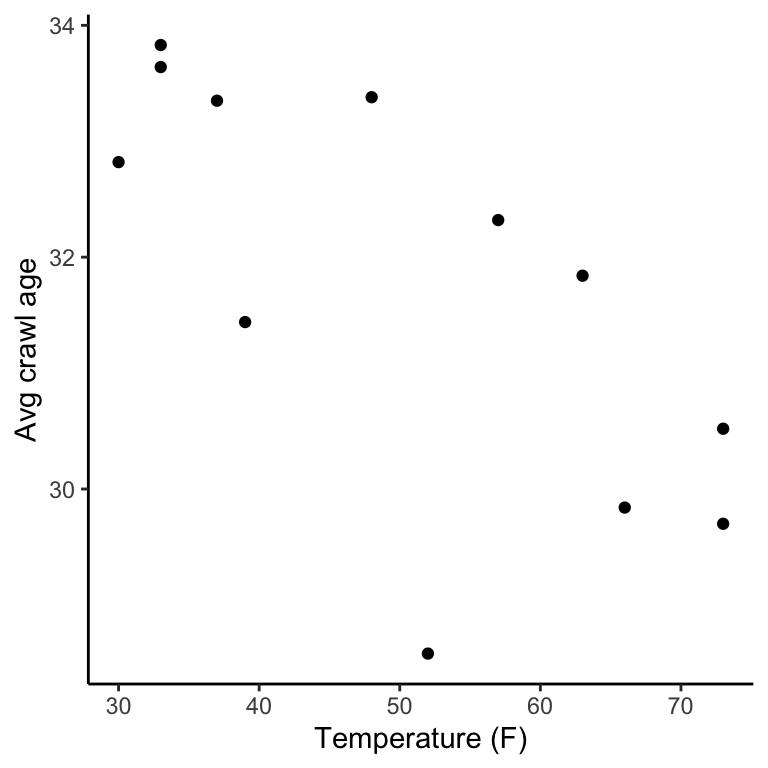
\includegraphics{Applied-regression-analysis_files/figure-latex/unnamed-chunk-3-1.pdf}

However, it would be convenient to also have a \emph{quantitative} measure summarizing the degree or strength of the linear relationship.

\hypertarget{covariance}{%
\subsection{Covariance}\label{covariance}}

One possible quantitative measure of linear association we could use is \textbf{covariance}.
* Covariance between \(X-1\) and \(Y\):
\[
c_{Y1} = \frac{\sum{(X_{1i} - \bar{X_1})(Y_{i} - \bar{Y})}}{n-1} = -19.53
\]

\begin{itemize}
\tightlist
\item
  However, the covariance is \emph{not} independent of the scales of \(X_1\) and \(Y\). Thus, its magnitude as affected by both the strength of linear relationship \emph{and} the scales of the variables.

  \begin{itemize}
  \tightlist
  \item
    So if \(Y\) has variance of 1,000,000 and \(X_1\) has a variance of10, it is hard to know what covariance means because of the different scales
  \end{itemize}
\item
  Consequently, the covariance is \emph{not} bounded by -1 and +1.
\end{itemize}

\hypertarget{pearson-correlation-coefficient}{%
\subsection{Pearson correlation coefficient}\label{pearson-correlation-coefficient}}

So we would like a quantitative measure summarizing the degree or strength of the linear relationship. \emph{And} we would like that measure to \emph{not} change with ann arbitrary change in units of the variables\ldots{}

We can eliminate scale issues for \(X_1\) and \(Y\) by dividing by the standard deviations of both variables, yielding the \textbf{Peaarson correlation coefficient:}
\[
r_{Y1} = \frac{\sum{(X_{1i} - \bar{X_1})(Y_{i} - \bar{Y})}}{(n-1)sd_{1}sd_{Y}}
\]

or, equivalently (\(c_{Y1}\)) was defined as the covariance:
\[
r_{Y1} = \frac{c_{Y1}}{sd_{1}sd_{Y}}
\]

\begin{itemize}
\item
  The correlation is independent of scales of measurements because it uses standardized scores(\(z_1\) and \(z_Y\)) which are not altered by linear transformation of raw scores (\(X_1\) and \(Y\)).
  \[
  r_{Y1} = \frac{\sum{(X_{1i} - \bar{X_1})(Y_{i} - \bar{Y})}}{(n-1)sd_{1}sd_{Y}} \\
  = r_{Y1} = \frac{\sum{z_{1i}z_{Yi}}}{n -1}
  \]
\item
  where \(z_{1i}\) and \(z_{Yi}\) are standardized scores (z-scores).
  \[
  z_{1i} = \frac{(X_{1i} - \bar{X_1})}{sd_1} \\
  z_{Yi} = \frac{(Y_{i} - \bar{Y})}{sd_Y}
  \]
\item
  Properties of standardized scores (z-scores)

  \begin{itemize}
  \tightlist
  \item
    Means are equal to 0
  \item
    Variance always equal to 1
  \end{itemize}
\item
  You can find the standardized score in R usinf the \texttt{scale()} function:
\end{itemize}

\begin{Shaded}
\begin{Highlighting}[]
\FunctionTok{scale}\NormalTok{(data\_crawl}\SpecialCharTok{$}\NormalTok{temp)}
\end{Highlighting}
\end{Shaded}

\begin{itemize}
\tightlist
\item
  Standardized sscores(z-scores) represent relative standing with respect to the mean.
\item
  Standardizing varibales does not change the ranking of scores

  \begin{itemize}
  \tightlist
  \item
    As you can see from the table below, the rank of z-scores are the same as the rank of raw scores.
  \item
    Raw scores that were above/below the mean corresponds with z-scores above/below 0.
  \end{itemize}
\end{itemize}

\begin{verbatim}
##   temp weeks        Z_1         Z_y       z1_zy
## 1   66 29.84  0.9807934 -1.09717461 -1.07610160
## 2   73 30.52  1.4190202 -0.71093886 -1.00883661
## 3   73 29.70  1.4190202 -1.17669374 -1.66975220
## 4   63 31.84  0.7929819  0.03881291  0.03077793
## 5   52 28.58  0.1043397 -1.81284675 -0.18915193
## 6   39 31.44 -0.7095101 -0.18838460  0.13366078
\end{verbatim}

\begin{itemize}
\item
  As well, points in standardized scores scatterplot retain the same relation to each other as in raw scores scatterplot. The underlying relationship remains the same.
  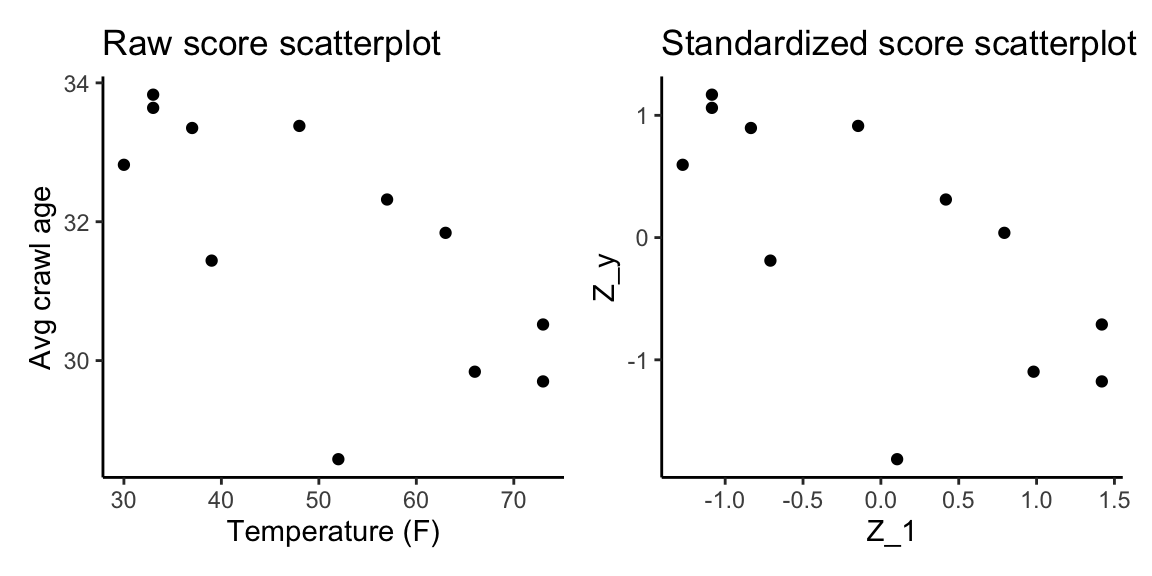
\includegraphics{Applied-regression-analysis_files/figure-latex/unnamed-chunk-6-1.pdf}
\item
  Now let's calculate the Pearson correlation using the \texttt{data\_crawl\$z1\_zy} column.
  \[
  r_{Y1} = \frac{\sum{z_{1i}z_{Yi}}}{n -1} = \frac{-7.71}{11} = -.70
  \]
\item
  Let us consider how this measure behaves under different relationships of variables:

  \begin{itemize}
  \tightlist
  \item
    Negative relationships: multiplying (+)(-) scores yields a negative sum of products

    \begin{itemize}
    \tightlist
    \item
      On average, being positive on x meant they were negative on y , meaning that we can expect a lot of negative values in the sum of products, thus resulting in a negative correlation.
    \end{itemize}
  \item
    Positive relationship: multiplying (+)(+) or (-)(-) yields a positive sum of products
  \item
    Zero relationship: yields zero sum of products
  \end{itemize}
\item
  correlations are bounded by +1 (perfect positive correlation) and -1 (perfect negative relationship) because the variance of a standardized variable is 1/-1.
\end{itemize}

\hypertarget{interpreting-a-pearson-correlation}{%
\section{Interpreting a Pearson correlation}\label{interpreting-a-pearson-correlation}}

\begin{itemize}
\tightlist
\item
  \textbf{Magnitude}: measures strength of linear relationship (larger absolute values are stronger)
\item
  \textbf{Sign} indicates direction of linear relationship
\item
  \textbf{Independent of scales} of measurement

  \begin{itemize}
  \tightlist
  \item
    This is because standardized scores (\(z_1\) and \(Z_Y\)) are noot alterated by linear transfoormatino of raw scores (\(X_1\) and \(Y\))
  \end{itemize}
\end{itemize}

\hypertarget{factors}{%
\chapter{Factors affecting correlation coefficients}\label{factors}}

\hypertarget{overview}{%
\section{Overview}\label{overview}}

Observed values of correlation coefficients are affected by a number of factors to be examined here:

\begin{longtable}[]{@{}lll@{}}
\toprule
\begin{minipage}[b]{(\columnwidth - 2\tabcolsep) * \real{0.19}}\raggedright
Factor\strut
\end{minipage} & \begin{minipage}[b]{(\columnwidth - 2\tabcolsep) * \real{0.24}}\raggedright
Consequences\strut
\end{minipage} & \begin{minipage}[b]{(\columnwidth - 2\tabcolsep) * \real{0.57}}\raggedright
Fix?\strut
\end{minipage}\tabularnewline
\midrule
\endhead
\begin{minipage}[t]{(\columnwidth - 2\tabcolsep) * \real{0.19}}\raggedright
Restriction of range\strut
\end{minipage} & \begin{minipage}[t]{(\columnwidth - 2\tabcolsep) * \real{0.24}}\raggedright
Usually reduce \emph{r}\strut
\end{minipage} & \begin{minipage}[t]{(\columnwidth - 2\tabcolsep) * \real{0.57}}\raggedright
``Correction for restriction of range''\strut
\end{minipage}\tabularnewline
\begin{minipage}[t]{(\columnwidth - 2\tabcolsep) * \real{0.19}}\raggedright
Outliers\strut
\end{minipage} & \begin{minipage}[t]{(\columnwidth - 2\tabcolsep) * \real{0.24}}\raggedright
Reduce or increase \emph{r}\strut
\end{minipage} & \begin{minipage}[t]{(\columnwidth - 2\tabcolsep) * \real{0.57}}\raggedright
Ideally, detect a priori\strut
\end{minipage}\tabularnewline
\begin{minipage}[t]{(\columnwidth - 2\tabcolsep) * \real{0.19}}\raggedright
Nonlinearity\strut
\end{minipage} & \begin{minipage}[t]{(\columnwidth - 2\tabcolsep) * \real{0.24}}\raggedright
Misleading \emph{r}\strut
\end{minipage} & \begin{minipage}[t]{(\columnwidth - 2\tabcolsep) * \real{0.57}}\raggedright
Ideally detect a priori (later lecture)\strut
\end{minipage}\tabularnewline
\begin{minipage}[t]{(\columnwidth - 2\tabcolsep) * \real{0.19}}\raggedright
Dichotomization\strut
\end{minipage} & \begin{minipage}[t]{(\columnwidth - 2\tabcolsep) * \real{0.24}}\raggedright
Usually reduce \emph{r}\strut
\end{minipage} & \begin{minipage}[t]{(\columnwidth - 2\tabcolsep) * \real{0.57}}\raggedright
Don't dichotomize (corrections avalible but not discussed here)\strut
\end{minipage}\tabularnewline
\bottomrule
\end{longtable}

\hypertarget{restriction-of-range}{%
\section{Restriction of range}\label{restriction-of-range}}

Within a given law school, there is a near-zero correlation between undergraduate GPA and LSAT scores. This is an instance f restriction of range affecting the correlation.

Suppose we are interested in the realtionship between \(X_1\) (UGPA) and \(Y\) (LSAT). However, individuals measured on \(X_1\) are \textbf{selected} to be in the sample (admitted to law school) only if their score on \(X_1\) is sufficiently high, exceeding some threshold.

In such situation, the range of \(X_1\) is said to be \emph{restricted}

It is useful ti distinguish between the correlation when selection had occured vs.~the correlation if no selection had occurred. The difference can be seen in the following representation of a scatterplot:

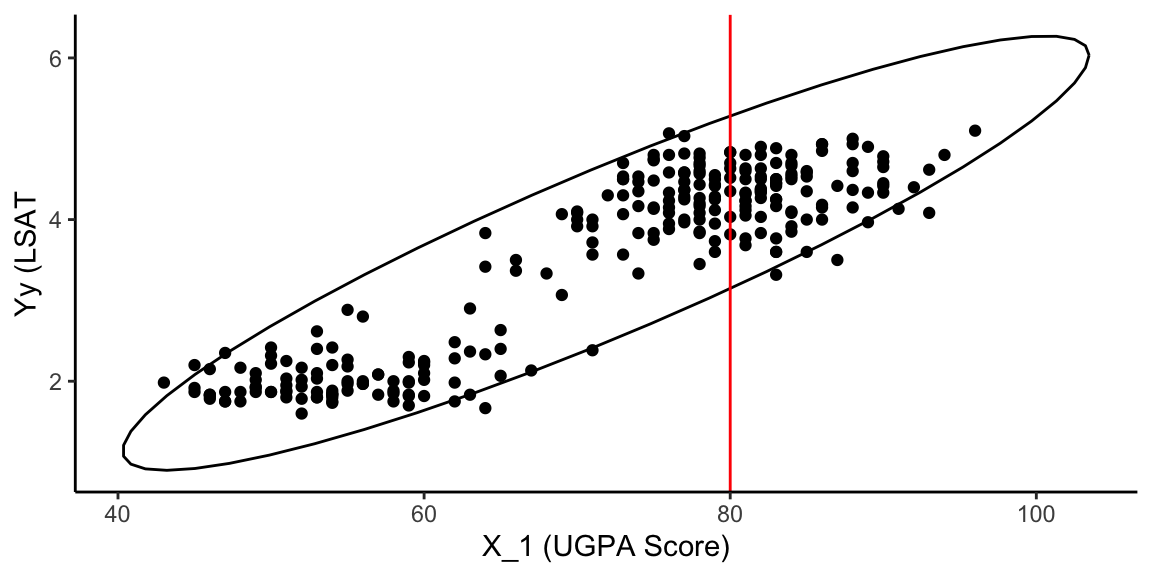
\includegraphics{Applied-regression-analysis_files/figure-latex/unnamed-chunk-8-1.pdf}

If no selection occurs, the relationship between \(X_1\) and \(Y\) is represented by the full ellipse. If selection occursm the relationship is represented by only the section of the ellipse beyoond the selection threshold on \(X_1\). It is evident that the correlation would be greater without selection.

This phenomenon impacts interpretation of correlations in s selection situation. After selecting for \(X_1\), the observed value of \(r_{Y1}\) may suggest a weaaker relationship then is actually present.

\hypertarget{correction-for-restriction-of-range}{%
\subsection{Correction for restriction of range}\label{correction-for-restriction-of-range}}

\hypertarget{outliers}{%
\section{Outliers}\label{outliers}}

\hypertarget{nonlinearity}{%
\section{Nonlinearity}\label{nonlinearity}}

\hypertarget{dichotomization}{%
\section{Dichotomization}\label{dichotomization}}

\hypertarget{methods}{%
\chapter{Methods}\label{methods}}

We describe our methods in this chapter.

\hypertarget{applications}{%
\chapter{Applications}\label{applications}}

Some \emph{significant} applications are demonstrated in this chapter.

\hypertarget{example-one}{%
\section{Example one}\label{example-one}}

\hypertarget{example-two}{%
\section{Example two}\label{example-two}}

\hypertarget{final-words}{%
\chapter{Final Words}\label{final-words}}

We have finished a nice book.

  \bibliography{book.bib,packages.bib}

\end{document}
